\documentclass[lettersize,journal]{IEEEtran}
\usepackage{amsmath,amsfonts,amssymb}
\usepackage{amsthm}
\newtheorem{theorem}{Theorem}
\usepackage{algorithmic}
\usepackage{algorithm}
\usepackage{array}
\usepackage[caption=false,font=normalsize,labelfont=sf,textfont=sf]{subfig}
\usepackage{textcomp}
\usepackage{stfloats}
\usepackage{url}
\usepackage{verbatim}
\usepackage{graphicx}
\usepackage{cite}
\usepackage{bm}
\usepackage{booktabs}
\usepackage{multirow}

\hyphenation{op-tical net-works semi-conduc-tor IEEE-Xplore ho-mo-to-py Tik-ho-nov non-lin-ear}

\begin{document}

\title{Tikhonov Integral Inversion for Simultaneous State and Input Estimation in Nonlinear Systems Using Dual Homotopy-Based Regressors}

\author{Rodolfo~H.~Rodrigo,~\IEEEmembership{Member,~IEEE,}
        Gustavo~Schweickardt,
        and~Daniel~H.~Pati\~no,~\IEEEmembership{Member,~IEEE}
\thanks{R.~H.~Rodrigo is with the Departamento Electromec\'anica, Facultad de Ingenier\'ia, Universidad Nacional de San Juan, San Juan J5400ARL, Argentina (e-mail: rodolfo\_rh@unsj.edu.ar).}
\thanks{G.~Schweickardt is with CONICET and Universidad Tecnol\'ogica Nacional, Paran\'a, Entre R\'ios, Argentina.}
\thanks{D.~H.~Pati\~no is with the Instituto de Autom\'atica (INAUT), Facultad de Ingenier\'ia, Universidad Nacional de San Juan, San Juan, Argentina.}
\thanks{Manuscript received XX XX, 2025; revised XX XX, 2025.}}

\markboth{IEEE Transactions on Systems, Man, and Cybernetics: Systems, Vol.~XX, No.~X, Month~2025}%
{Rodrigo \MakeLowercase{\textit{et al.}}: Tikhonov Integral Inversion for State and Input Estimation}

\maketitle

% =============================================================
% ABSTRACT (150-250 words, 5 elements)
% =============================================================
\begin{abstract}
Simultaneous estimation of states and unknown inputs in nonlinear dynamic systems is a long-standing challenge, particularly when numerical differentiation amplifies measurement noise and renders conventional inversion methods unusable. This paper introduces the Tikhonov Integral Inversion (TII), a method that addresses this problem through three synergistic elements. First, a dual regressor architecture is derived from the Homotopy Analysis Method (HAM), exploiting the observation that any implicit discrete equation can be resolved for \emph{any} of its variables, yielding a symmetric pair of direct (state prediction) and inverse (input reconstruction) regressors with identical convergence guarantees. Second, an integral formulation replaces noise-amplifying numerical differentiation with antiderivative-based evaluation, fundamentally changing the noise propagation characteristics of the inverse problem from ill-posed to well-posed. Third, first-difference Tikhonov regularization is applied to the integral inverse, yielding a tridiagonal linear system solvable in linear time. When integrated with an Extended Kalman Filter, the direct regressor serves as the state transition model while TII provides input estimation with quantified uncertainty. The method is validated on a DC motor benchmark with nonlinear magnetic saturation, where it consistently outperforms differential inversion, unregularized integral inversion, and EKF-based alternatives across all tested noise levels, with improvements spanning one to two orders of magnitude.
\end{abstract}

\begin{IEEEkeywords}
Tikhonov regularization, unknown input estimation, homotopy analysis method, nonlinear Kalman filtering, integral inversion, magnetic saturation.
\end{IEEEkeywords}

% =============================================================
% I. INTRODUCTION (800-1200 words, 8-15 cites)
% =============================================================
\section{Introduction}
\label{sec:intro}

\IEEEPARstart{T}{he} simultaneous estimation of states and unknown inputs in nonlinear dynamic systems is a fundamental problem in control engineering, fault diagnosis, and system monitoring \cite{gillijns2007, hou1998}. In many practical scenarios, not all system variables are directly measurable, and some inputs---such as disturbance forces, actuator faults, or unmeasured loads---must be inferred from available sensor data. This class of problems has attracted sustained attention in the systems, man, and cybernetics community because it lies at the intersection of observer design, system identification, and inverse problems \cite{simon2006, ljung1987}.

The challenge is particularly acute in nonlinear systems where the relationship between states and inputs is implicit. For instance, in electromechanical drives, the angular velocity may be measured by an encoder, but the armature current---which generates the electromagnetic torque---must be inferred from the electrical dynamics. When these dynamics include nonlinear effects such as magnetic saturation, the estimation problem becomes mathematically implicit: the unknown variable appears inside a nonlinear function that cannot be algebraically inverted \cite{krause2013, boldea2010}.

The classical approach to joint state--input estimation augments the state vector with the unknown input, modeled as a random walk $u_{k+1} = u_k + w_k$, and applies the Extended Kalman Filter (EKF) or the Unscented Kalman Filter (UKF) to the augmented system \cite{kitanidis1987, gillijns2007, fang2012}. While effective in certain regimes, this approach has three well-documented limitations: (i)~the input must vary slowly relative to the sampling period; (ii)~the noise covariance $Q_u$ of the random walk must be tuned manually, creating a trade-off between tracking speed and estimation noise; and (iii)~the augmented state dimension increases the computational cost of the Kalman gain calculation \cite{hsieh2000, yong2016}.

An alternative paradigm is model inversion: given a plant model and measured outputs, one solves for the input. For linear systems this reduces to algebraic manipulation \cite{moylan1977}; for nonlinear systems, iterative numerical methods or neural-network-based inverse models are required \cite{hunt1996, narendra1990}. However, all differential-based inversion methods face a fundamental limitation: when measurements are corrupted by noise, numerical differentiation amplifies the noise by a factor proportional to $1/T$ (where $T$ is the sampling period), rendering the reconstruction unusable at practical sampling rates \cite{chartrand2011, hanke2001}. This is a manifestation of the classical ill-posedness of numerical differentiation, extensively studied in the regularization theory literature \cite{engl1996, tikhonov1977}.

In \cite{rodrigo2021rpic}, we introduced the Homotopy-Based Functional Neural Network (HFNN), which uses the Homotopy Analysis Method (HAM) \cite{liao2003} to convert implicit nonlinear discrete equations into explicit algebraic regressors. The present paper extends that work with three contributions:

\begin{enumerate}
    \item \textbf{Variable-agnostic HAM regressors.} We prove that HAM produces explicit regressors for \emph{any} variable of the implicit equation $F=0$ (Theorem~\ref{thm:agnostic}), yielding a symmetric direct/inverse pair with identical convergence guarantees.
    
    \item \textbf{Integral formulation.} By integrating the governing ODE between consecutive samples, the inverse regressor replaces noise-amplifying numerical differentiation with smooth antiderivative evaluation, reducing noise gain from $O(\sigma/T)$ to $O(\sigma)$.
    
    \item \textbf{Tikhonov Integral Inversion (TII).} The integral inverse is formulated as a regularized least-squares problem with first-difference penalty, yielding a tridiagonal system solvable in $O(n)$ time. TII combines intrinsic noise suppression from integration with global smoothness from regularization.
\end{enumerate}

When combined with an EKF, the direct regressor serves as the state transition model while TII provides filtered input estimation with analytically propagated uncertainty. The architecture eliminates state augmentation, random-walk hypotheses, and numerical differentiation.

The approach is validated on a DC motor with nonlinear inductance $L(i)$ due to magnetic saturation, comparing seven estimation strategies across four noise levels. At measurement noise $\sigma = 0.1$, TII achieves a voltage reconstruction RMSE of $0.102$~V---a 166-fold improvement over the 3-point differential inverse ($16.89$~V), 92-fold over the unregularized integral ($9.33$~V), and 33-fold over EKF with derivative-based reconstruction ($3.38$~V). At the highest noise level ($\sigma = 0.5$), TII maintains RMSE~$= 0.151$~V (309-fold improvement) while derivative-based EKF methods diverge entirely.

The remainder of this paper is organized as follows. Section~\ref{sec:background} introduces the necessary theoretical tools. Section~\ref{sec:related} surveys related work. Section~\ref{sec:problem} formalizes the problem. Section~\ref{sec:method} presents the proposed method. Section~\ref{sec:experiments} describes the experimental setup and results. Section~\ref{sec:discussion} discusses findings and limitations. Section~\ref{sec:conclusion} concludes.

% =============================================================
% II. BACKGROUND (600-1000 words, 5-10 cites, 3-6 eqs)
% =============================================================
\section{Background}
\label{sec:background}

This section reviews the three theoretical pillars on which the proposed method is built: the Homotopy Analysis Method, Tikhonov regularization theory, and the Extended Kalman Filter.

\subsection{Homotopy Analysis Method (HAM)}

The Homotopy Analysis Method, developed by Liao \cite{liao2003, liao2012}, provides a general framework for solving nonlinear equations by embedding them in a continuous deformation from a known solution to the desired one. Given an implicit equation $F(\mathbf{z}) = 0$, HAM constructs a homotopy
\begin{equation}
\label{eq:homotopy}
\mathcal{H}(\mathbf{z}; q) = (1 - q)[L(\mathbf{z}) - L(\mathbf{z}_0)] + q\,c_0\,F(\mathbf{z}) = 0,
\end{equation}
where $q \in [0,1]$ is the embedding parameter, $L$ is an auxiliary linear operator, $\mathbf{z}_0$ is an initial approximation, and $c_0$ is a convergence-control parameter. When $q = 0$, the solution is the initial guess; when $q = 1$, the original equation is recovered. The solution is expanded as a power series in $q$, and evaluating at $q = 1$ yields successive approximations. A key advantage of HAM over perturbation methods is that convergence can be guaranteed for strongly nonlinear problems by appropriate choice of $c_0$ \cite{liao2003}.

For the Newton homotopy (taking $L = F'$, $c_0 = 1$), the first two corrections to an initial guess $z^{(0)}$ for a scalar equation $g(z) = 0$ are:
\begin{align}
\zeta_1 &= -\frac{g(z^{(0)})}{g'(z^{(0)})}, \label{eq:newton}\\
\zeta_2 &= -\frac{g(z^{(0)})^2 \, g''(z^{(0)})}{2\,g'(z^{(0)})^3}. \label{eq:halley}
\end{align}
The first term is the Newton correction; the second is the Halley correction, which accounts for curvature and achieves cubic convergence \cite{householder1970}.

\subsection{Tikhonov Regularization}

Tikhonov regularization \cite{tikhonov1977} addresses ill-posed inverse problems by introducing a penalty term that constrains the solution. For a linear system $\mathbf{A}\mathbf{x} = \mathbf{b}$ with noisy right-hand side, the regularized solution minimizes
\begin{equation}
\label{eq:tikhonov_general}
\|\mathbf{A}\mathbf{x} - \mathbf{b}\|^2 + \lambda\,\|\mathbf{L}\mathbf{x}\|^2,
\end{equation}
where $\lambda > 0$ is the regularization parameter and $\mathbf{L}$ is a regularization operator---commonly the identity (zeroth order) or a finite-difference matrix (first or second order) \cite{hansen1998}. The parameter $\lambda$ balances data fidelity against solution smoothness. Standard selection methods include the L-curve criterion \cite{hansen1992}, Generalized Cross-Validation (GCV) \cite{golub1979}, and the discrepancy principle \cite{engl1996}.

\subsection{Extended Kalman Filter}

The Extended Kalman Filter \cite{simon2006} extends the classical Kalman filter to nonlinear systems by linearizing the state transition and measurement models around the current estimate. For a continuous-time system with discrete measurements, the prediction step integrates the nonlinear dynamics (e.g., via Runge--Kutta), while the covariance is propagated using the Jacobian $\mathbf{F}_k = \mathbf{I} + \mathbf{A}_k T$, where $\mathbf{A}_k = \partial \mathbf{f}/\partial \mathbf{x}$ is the analytical Jacobian of the continuous-time dynamics \cite{wan2000}. The update step fuses the prediction with the measurement using the Kalman gain. The Joseph form of the covariance update is preferred for numerical stability \cite{simon2006}:
\begin{equation}
\label{eq:joseph}
\mathbf{P}_{k|k} = (\mathbf{I} - \mathbf{K}_k\mathbf{H})\mathbf{P}_{k|k-1}(\mathbf{I} - \mathbf{K}_k\mathbf{H})^\top + \mathbf{K}_k R_v \mathbf{K}_k^\top.
\end{equation}

% =============================================================
% III. RELATED WORK (900-1300 words, 20-40 cites, 1 table)
% =============================================================
\section{Related Work}
\label{sec:related}

The problem of simultaneous state and input estimation has been addressed through several distinct paradigms. We organize the literature into four categories: augmented-state Kalman methods, model-inversion approaches, regularization-based methods, and neural/functional network approaches.

\subsection{Augmented-State Kalman Filtering}

The most widely used approach models the unknown input as an additional state variable with random-walk dynamics and applies the EKF or UKF to the augmented system. Kitanidis \cite{kitanidis1987} established the theoretical foundations for unbiased minimum-variance estimation. Gillijns and De Moor \cite{gillijns2007} extended this to the discrete-time case and proposed recursive algorithms for linear systems. Fang et al.\ \cite{fang2012} analyzed stability conditions for simultaneous input and state estimation. Hsieh \cite{hsieh2000} applied the augmented EKF to fault detection in nonlinear systems, while Yong et al.\ \cite{yong2016} provided a unified framework for joint estimation with known input distribution.

The augmented-state approach has known limitations: the random-walk model introduces lag when the input changes rapidly, the covariance $Q_u$ requires manual tuning, and the augmented dimension increases computational cost \cite{darouach1997}. Palanthandalam-Madapusi and Bernstein \cite{palanthandalam2007} showed that unbiased estimation requires specific rank conditions on the system matrices, which are not always satisfied in practice.

\subsection{Model Inversion and Observer-Based Methods}

An alternative paradigm reconstructs the input directly from the measured output and a plant model. For linear systems, Moylan \cite{moylan1977} established conditions for exact model inversion. Hou and Patton \cite{hou1998} developed unknown input observers (UIOs) that estimate the state while decoupling the unknown input. Floquet and Barbot \cite{floquet2007} used sliding-mode observers for robust input reconstruction in the presence of modeling uncertainties.

For nonlinear systems, model inversion generally requires numerical differentiation of measured signals, which amplifies noise \cite{chartrand2011}. Sundaram and Hadjicostis \cite{sundaram2007} analyzed the fundamental limitations of delayed input reconstruction, showing that $d$ steps of delay are needed for $d$th-order systems. More recently, Shi et al.\ \cite{shi2016} proposed an $H_\infty$ approach for simultaneous estimation in nonlinear systems, but the method requires solving LMIs that become intractable for high-dimensional problems.

\subsection{Regularization Approaches for Inverse Problems}

The connection between input estimation and classical inverse problems has been recognized but underexplored in the control literature. Numerical differentiation is a canonical ill-posed problem \cite{hanke2001}, and Tikhonov regularization \cite{tikhonov1977} is the standard remedy. Chartrand \cite{chartrand2011} proposed total-variation regularization for numerical differentiation of noisy data, achieving noise suppression without excessive smoothing of discontinuities. Hansen \cite{hansen1998, hansen1992} developed the L-curve method for automated selection of the regularization parameter. Golub et al.\ \cite{golub1979} introduced GCV as an alternative that does not require knowledge of the noise level.

In the systems and control context, Orjuela et al.\ \cite{orjuela2019} applied Tikhonov regularization to force identification in structural dynamics, but their formulation operates on the differential (not integral) form of the equations, limiting noise suppression. The idea of reformulating the inverse problem in integral form---which is the key contribution of this paper---has not been explored for input estimation in nonlinear systems.

\subsection{Neural and Functional Network Approaches}

Neural networks have been extensively used for system identification and inverse modeling. Narendra and Parthasarathy \cite{narendra1990} provided the foundational framework for neural identification of dynamical systems. Hunt et al.\ \cite{hunt1996} surveyed neural approaches to control, including inverse models. Castillo et al.\ \cite{castillo1998} introduced functional networks as an alternative to neural networks, embedding known functional structure into the model architecture.

More recently, physics-informed neural networks (PINNs) \cite{raissi2019} have gained attention for solving forward and inverse problems in dynamical systems by embedding the governing PDE as a loss term. However, PINNs require extensive training data and computational resources, and provide no convergence guarantees for the inverse problem. Brunton et al.\ \cite{brunton2016} proposed sparse identification of nonlinear dynamics (SINDy), which discovers governing equations from data but does not address the input estimation problem directly. Chen et al.\ \cite{chen2018} introduced neural ODEs for continuous-depth models, enabling differentiable simulation, but again without addressing inverse estimation.

The homotopy-based approach proposed in \cite{rodrigo2021rpic} and extended in this paper occupies a unique position: it provides closed-form algebraic regressors with analytical derivatives, convergence guarantees, and compatibility with classical filtering---advantages that purely data-driven methods lack.

\subsection{Summary and Gap Analysis}

Table~\ref{tab:related} summarizes the key approaches and their limitations, motivating the proposed TII method.

\begin{table}[!t]
\centering
\caption{Comparison of Approaches for Unknown Input Estimation}
\label{tab:related}
\begin{tabular}{p{2.7cm}ccp{2.8cm}}
\toprule
Method & Causal & Nonlinear & Key Limitation \\
\midrule
Augmented EKF \cite{gillijns2007} & Yes & Yes & Random-walk assumption, $Q_u$ tuning \\
UIO \cite{hou1998} & Yes & Limited & Rank conditions, linear-only \\
Sliding-mode \cite{floquet2007} & Yes & Yes & Chattering, tuning \\
$H_\infty$ \cite{shi2016} & Yes & Yes & LMI scalability \\
Tikhonov (diff.) \cite{orjuela2019} & No & Limited & Noise amplification from differentiation \\
PINNs \cite{raissi2019} & No & Yes & Training cost, no guarantees \\
SINDy \cite{brunton2016} & No & Yes & Forward-only, no input est. \\
\midrule
\textbf{TII (proposed)} & \textbf{No} & \textbf{Yes} & \textbf{Batch processing, $\lambda$ selection} \\
\bottomrule
\end{tabular}
\end{table}

The gap in the literature is clear: no existing method combines (a)~a principled noise-suppressing integral formulation, (b)~algebraic regressors with analytical derivatives, and (c)~Tikhonov regularization with $O(n)$ computational cost. TII addresses this gap.

% =============================================================
% IV. PROBLEM FORMULATION (400-700 words, 4-8 eqs)
% =============================================================
\section{Problem Formulation}
\label{sec:problem}

Consider a nonlinear dynamic system described by the coupled ODEs:
\begin{align}
J\,\frac{d\omega}{dt} &= K_t\,i - b\,\omega - N_{\text{load}}(\omega), \label{eq:mech} \\
L(i)\,\frac{di}{dt} &= u - R\,i - K_e\,\omega, \label{eq:elec}
\end{align}
where $\omega$ is the angular velocity (measurable), $i$ is the armature current (to be estimated), $u$ is the input voltage (unknown), $J$ is the moment of inertia, $b$ is viscous friction, $K_t$ and $K_e$ are motor constants, $R$ is armature resistance, $N_{\text{load}}(\omega)$ is a nonlinear load torque, and $L(i)$ is a current-dependent inductance modeling magnetic saturation.

The measurement model provides noisy observations of only the angular velocity:
\begin{equation}
\label{eq:meas}
z_k = \omega(t_k) + v_k, \quad v_k \sim \mathcal{N}(0, \sigma^2),
\end{equation}
sampled at period $T$, with $k = 0, 1, \ldots, n-1$.

The estimation problem consists of three objectives:
\begin{enumerate}
    \item[(O1)] \textbf{State estimation:} Given $\{z_k\}$, estimate the filtered state trajectory $\{\hat{\omega}_k, \hat{i}_k\}$.
    \item[(O2)] \textbf{Input reconstruction:} From the estimated states, reconstruct the unknown input $\{u_k\}$.
    \item[(O3)] \textbf{Uncertainty quantification:} Provide confidence bounds on both state and input estimates.
\end{enumerate}

The fundamental difficulty lies in objective (O2). Discretizing \eqref{eq:elec} with finite differences yields:
\begin{equation}
\label{eq:inv_diff}
\hat{u}_k = L(i_k)\,\frac{d_p[i]_k}{T} + R\,i_k + K_e\,\omega_k,
\end{equation}
where $d_p[i]_k$ denotes a $p$-point backward difference stencil. When $i_k$ is corrupted by noise $\epsilon_k$ with standard deviation $\sigma$, the noise in the estimated input scales as:
\begin{equation}
\label{eq:noise_amp}
\text{Var}(\hat{u}_k) \propto \frac{c_p^2 \, \sigma^2}{T^2},
\end{equation}
where $c_p$ is a stencil-dependent constant ($c_1 = 1$, $c_2 = \sqrt{5/2}$, $c_3 = \sqrt{35/6}$). For $T = 0.1$~ms and $\sigma = 0.1$, this yields noise amplification of order $10^4$---the estimated input is pure noise.

The goal of this paper is to develop a method that achieves objectives (O1)--(O3) without the noise amplification inherent in \eqref{eq:inv_diff}.

% =============================================================
% V. PROPOSED METHOD (1500-2200 words, 10-20 eqs, 2-4 figs)
% =============================================================
\section{Proposed Method: Tikhonov Integral Inversion}
\label{sec:method}

The proposed method comprises three components: (A)~variable-agnostic HAM regressors, (B)~the integral formulation, and (C)~Tikhonov regularization. Together, these form the TII architecture.

\subsection{Variable-Agnostic HAM Regressors}

\begin{theorem}[Variable-agnostic HAM regressor]
\label{thm:agnostic}
Let $F(z_1, \ldots, z_n) = 0$ be an implicit equation with $F \in C^2$. For any index $j$ such that $\partial F / \partial z_j \neq 0$ at the expansion point, the HAM regressor
\begin{equation}
\label{eq:ham_regressor}
\hat{z}_j = z_j^{(0)} + \zeta_1 + \zeta_2,
\end{equation}
with $\zeta_1, \zeta_2$ given by \eqref{eq:newton}--\eqref{eq:halley}, produces an explicit expression for $z_j$ as a function of the remaining variables. The truncation error, convergence conditions, and rational structure are identical regardless of the choice of $j$.
\end{theorem}

\begin{proof}
The construction depends only on $g(z_j) = F|_{z_{\neq j} \text{ fixed}}$ and its derivatives. Convergence is governed by the Cauchy--Hadamard criterion applied to $g$, depending on analyticity of $F$ with respect to $z_j$ and the non-degeneracy $g'(z_j^{(0)}) \neq 0$. These hold generically for any $z_j$. The truncation error is $O(|g'''|/|g'|^5)$, independent of the physical meaning of $z_j$.
\end{proof}

Applied to the discretized system \eqref{eq:mech}--\eqref{eq:elec}, Theorem~\ref{thm:agnostic} yields:
\begin{itemize}
    \item A \textbf{direct regressor} resolving for $(\omega_k, i_k)$ given past states and input (state prediction), as developed in \cite{rodrigo2021rpic}.
    \item An \textbf{inverse regressor} resolving for $u_k$ given measured states (input reconstruction).
\end{itemize}
Both share identical mathematical structure and analytical derivatives, enabling seamless integration with the EKF.

\subsection{Integral Formulation}

The key insight is that the electrical equation \eqref{eq:elec} can be \emph{integrated} between consecutive sample times rather than differentiated. Integrating from $t_{k-1}$ to $t_k$:
\begin{equation}
\label{eq:int_elec}
\int_{t_{k-1}}^{t_k} L(i)\,\frac{di}{dt}\,dt = \int_{t_{k-1}}^{t_k} [u - R\,i - K_e\,\omega]\,dt.
\end{equation}

The left-hand side evaluates exactly via the chain rule:
\begin{equation}
\label{eq:antideriv}
\int_{i_{k-1}}^{i_k} L(s)\,ds = \Phi(i_k) - \Phi(i_{k-1}),
\end{equation}
where $\Phi(i) = \int L(i)\,di$ is the antiderivative. For the saturation model $L(i) = L_0/(1 + (i/I_{\text{sat}})^2)$:
\begin{equation}
\label{eq:Phi}
\Phi(i) = L_0 \, I_{\text{sat}} \, \arctan(i/I_{\text{sat}}).
\end{equation}

The right-hand side is approximated by the trapezoidal rule (A-stable, $O(T^2)$), yielding:
\begin{equation}
\label{eq:inv_integral}
\boxed{
\hat{u}_k = \frac{\Phi(i_k) - \Phi(i_{k-1})}{T} + \frac{R}{2}(i_{k-1} + i_k) + \frac{K_e}{2}(\omega_{k-1} + \omega_k).
}
\end{equation}

The noise properties of \eqref{eq:inv_integral} differ fundamentally from the differential form \eqref{eq:inv_diff}:

\begin{enumerate}
    \item The antiderivative $\Phi(i) = L_0 I_{\text{sat}} \arctan(i/I_{\text{sat}})$ is globally Lipschitz with constant $L_0$. Noise propagates as $|\Phi(i+\epsilon) - \Phi(i)| \leq L_0|\epsilon|$, bounded independently of $T$.
    
    \item The resistive and back-EMF terms use \emph{averaging} (trapezoidal rule), reducing noise by $1/\sqrt{2}$ compared to differencing.
    
    \item The overall noise gain is $O(\sigma)$, compared to $O(\sigma/T)$ for the differential formulation---an improvement factor of $O(1/T)$ that grows with sampling rate.
\end{enumerate}

The same integration procedure applies to \eqref{eq:mech}, yielding the \textbf{direct integral regressor}:
\begin{equation}
\label{eq:direct_integral}
J(\omega_k - \omega_{k-1}) + \frac{T}{2}[h(\omega_{k-1}, i_{k-1}) + h(\omega_k, i_k)] = 0,
\end{equation}
where $h(\omega, i) = b\omega + N_{\text{load}}(\omega) - K_t\,i$. This implicit system is solved by two Newton iterations, requiring only one initial condition per variable (vs.\ two for the 3-point stencil) and with Jacobian dominated by $J$ and $L(i)$ rather than $1/T^2$.

\subsection{Tikhonov Regularization on the Integral Inverse}

While the integral formulation \eqref{eq:inv_integral} suppresses noise compared to differentiation, it still propagates measurement noise point-by-point. Global regularization provides a second layer of suppression.

Given $n$ samples of noisy $(\omega_k, i_k)$, define the data vector $\mathbf{b} \in \mathbb{R}^{n-1}$ with $b_k$ given by \eqref{eq:inv_integral}. The TII solves:
\begin{equation}
\label{eq:tii}
\min_{\mathbf{u}} \;\|\mathbf{u} - \mathbf{b}\|^2 + \lambda \|\mathbf{D}\mathbf{u}\|^2,
\end{equation}
where $\mathbf{D} \in \mathbb{R}^{(n-2)\times(n-1)}$ is the first-difference matrix and $\lambda > 0$ controls the smoothness--fidelity trade-off. The normal equations are:
\begin{equation}
\label{eq:normal}
(\mathbf{I} + \lambda\,\mathbf{D}^\top \mathbf{D})\,\mathbf{u} = \mathbf{b}.
\end{equation}

The matrix $\mathbf{D}^\top\mathbf{D}$ is symmetric tridiagonal with diagonal $[1, 2, \ldots, 2, 1]$ and off-diagonal $[-1, \ldots, -1]$. Therefore $\mathbf{I} + \lambda\mathbf{D}^\top\mathbf{D}$ is symmetric positive definite and tridiagonal, solvable by the Thomas algorithm in $O(n)$ operations \cite{golub2013}. The solution time is consistently below 1~ms for $n = 2000$.

Key properties of TII:
\begin{enumerate}
    \item \textbf{Linearity:} $\mathbf{u} = \mathbf{S}_\lambda\mathbf{b}$ where $\mathbf{S}_\lambda = (\mathbf{I} + \lambda\mathbf{D}^\top\mathbf{D})^{-1}$ is a smoothing matrix.
    \item \textbf{Two-layer suppression:} Integration (first layer) + Tikhonov smoothing (second layer).
    \item \textbf{No slow-variation assumption:} Unlike random-walk models, $\lambda$ controls smoothness without assuming the input varies slowly.
    \item \textbf{$O(n)$ cost:} Tridiagonal solve, compared to $O(n^3)$ for generic Tikhonov.
\end{enumerate}

\subsection{EKF Integration}

The complete estimation architecture operates as follows:

\textbf{State space:} $\mathbf{x} = [\omega, i]^\top$. Measurement: $z_k = \omega_k + v_k$.

\textbf{Prediction:} The EKF integrates \eqref{eq:mech}--\eqref{eq:elec} via RK4 with the estimated input $\hat{u}_{k-1}$. The covariance is propagated using the analytical Jacobian:
\begin{equation}
\label{eq:jac_A}
\mathbf{A} = \begin{bmatrix}
-(b + N'_{\text{load}})/J & K_t/J \\[4pt]
-K_e/L(i) & -R/L(i) - \dot{i}\,L'(i)/L(i)
\end{bmatrix},
\end{equation}
discretized as $\mathbf{F}_k = \mathbf{I} + \mathbf{A}_k T$.

\textbf{Update:} Standard Kalman update with $\mathbf{H} = [1, 0]$ and Joseph-form covariance \eqref{eq:joseph}.

\textbf{Input reconstruction:} Two alternatives are compared:
\begin{align}
\hat{u}_k^{(\text{d})} &= R\hat{i}_k + L(\hat{i}_k)\frac{11\hat{i}_k - 18\hat{i}_{k-1} + 9\hat{i}_{k-2} - 2\hat{i}_{k-3}}{6T} + K_e\hat{\omega}_k, \label{eq:u_deriv}\\
\hat{u}_k^{(\text{i})} &= \frac{\Phi(\hat{i}_k) - \Phi(\hat{i}_{k-1})}{T} + \frac{R}{2}(\hat{i}_{k-1} + \hat{i}_k) + \frac{K_e}{2}(\hat{\omega}_{k-1} + \hat{\omega}_k). \label{eq:u_int_ekf}
\end{align}

The reconstructed input is fed back to the next prediction step. Uncertainty is propagated as $P_u = \mathbf{J}_G \mathbf{P}_{k|k} \mathbf{J}_G^\top$, where $\mathbf{J}_G = \partial\hat{u}/\partial\mathbf{x}$ is computed analytically.

\begin{algorithm}[!t]
\caption{TII Pipeline}
\label{alg:tii}
\begin{algorithmic}[1]
\REQUIRE Measurements $\{z_k\}_{k=0}^{n-1}$, motor parameters, $\lambda$
\STATE Initialize EKF: $\hat{\mathbf{x}}_0 = \mathbf{0}$, $\mathbf{P}_0 = \mathbf{I}$
\FOR{$k = 1$ to $n-1$}
    \STATE EKF predict: $\hat{\mathbf{x}}_{k|k-1} = \text{RK4}(\hat{\mathbf{x}}_{k-1|k-1}, \hat{u}_{k-1}, T)$
    \STATE EKF update: $\hat{\mathbf{x}}_{k|k}$ from $z_k$
    \STATE Integral inverse: $b_k$ via \eqref{eq:inv_integral} from $\hat{\mathbf{x}}_{k|k}$
    \STATE Causal feedback: $\hat{u}_k = b_k$ (for next EKF step)
\ENDFOR
\STATE Solve TII: $(\mathbf{I} + \lambda\mathbf{D}^\top\mathbf{D})\mathbf{u} = \mathbf{b}$ (Thomas algorithm)
\RETURN $\{\hat{\omega}_k, \hat{i}_k, \hat{u}_k\}$
\end{algorithmic}
\end{algorithm}

% =============================================================
% VI. EXPERIMENTS (1200-1800 words, 2-5 figs, 2-4 tables)
% =============================================================
\section{Experiments}
\label{sec:experiments}

\subsection{System and Ground Truth}

The case study uses a DC motor governed by \eqref{eq:mech}--\eqref{eq:elec} with parameters in Table~\ref{tab:params}. The nonlinear functions are $L(i) = L_0/(1 + (i/I_{\text{sat}})^2)$ and $N_{\text{load}}(\omega) = c\omega^2$, with antiderivative $\Phi(i) = L_0 I_{\text{sat}} \arctan(i/I_{\text{sat}})$.

\begin{table}[!t]
\centering
\caption{Motor Parameters}
\label{tab:params}
\begin{tabular}{llll}
\toprule
Symbol & Value & Unit & Description \\
\midrule
$R$ & 1.0 & $\Omega$ & Armature resistance \\
$K_e, K_t$ & 0.1 & V$\cdot$s/rad, N$\cdot$m/A & Motor constants \\
$J$ & 0.001 & kg$\cdot$m$^2$ & Inertia \\
$b$ & 0.01 & N$\cdot$m$\cdot$s/rad & Viscous friction \\
$L_0$ & 0.01 & H & Unsaturated inductance \\
$I_{\text{sat}}$ & 10.0 & A & Saturation current \\
$c$ & $10^{-5}$ & -- & Load torque coeff. \\
\bottomrule
\end{tabular}
\end{table}

True trajectories are generated by RK4 integration with step $\Delta t = 10^{-6}$~s. The input is a step voltage: $u = 0$~V for $t \leq 5$~ms and $u = 12$~V for $t > 5$~ms. The solution is downsampled to $T = 0.1$~ms ($n = 2000$ samples, $t_f = 0.2$~s). Independent Gaussian noise $\mathcal{N}(0, \sigma^2)$ is added to both $\omega_k$ and $i_k$, with $\sigma \in \{0.01, 0.05, 0.1, 0.5\}$. Fig.~\ref{fig:ground_truth} shows the ground truth trajectories.

\begin{figure}[!t]
\centering
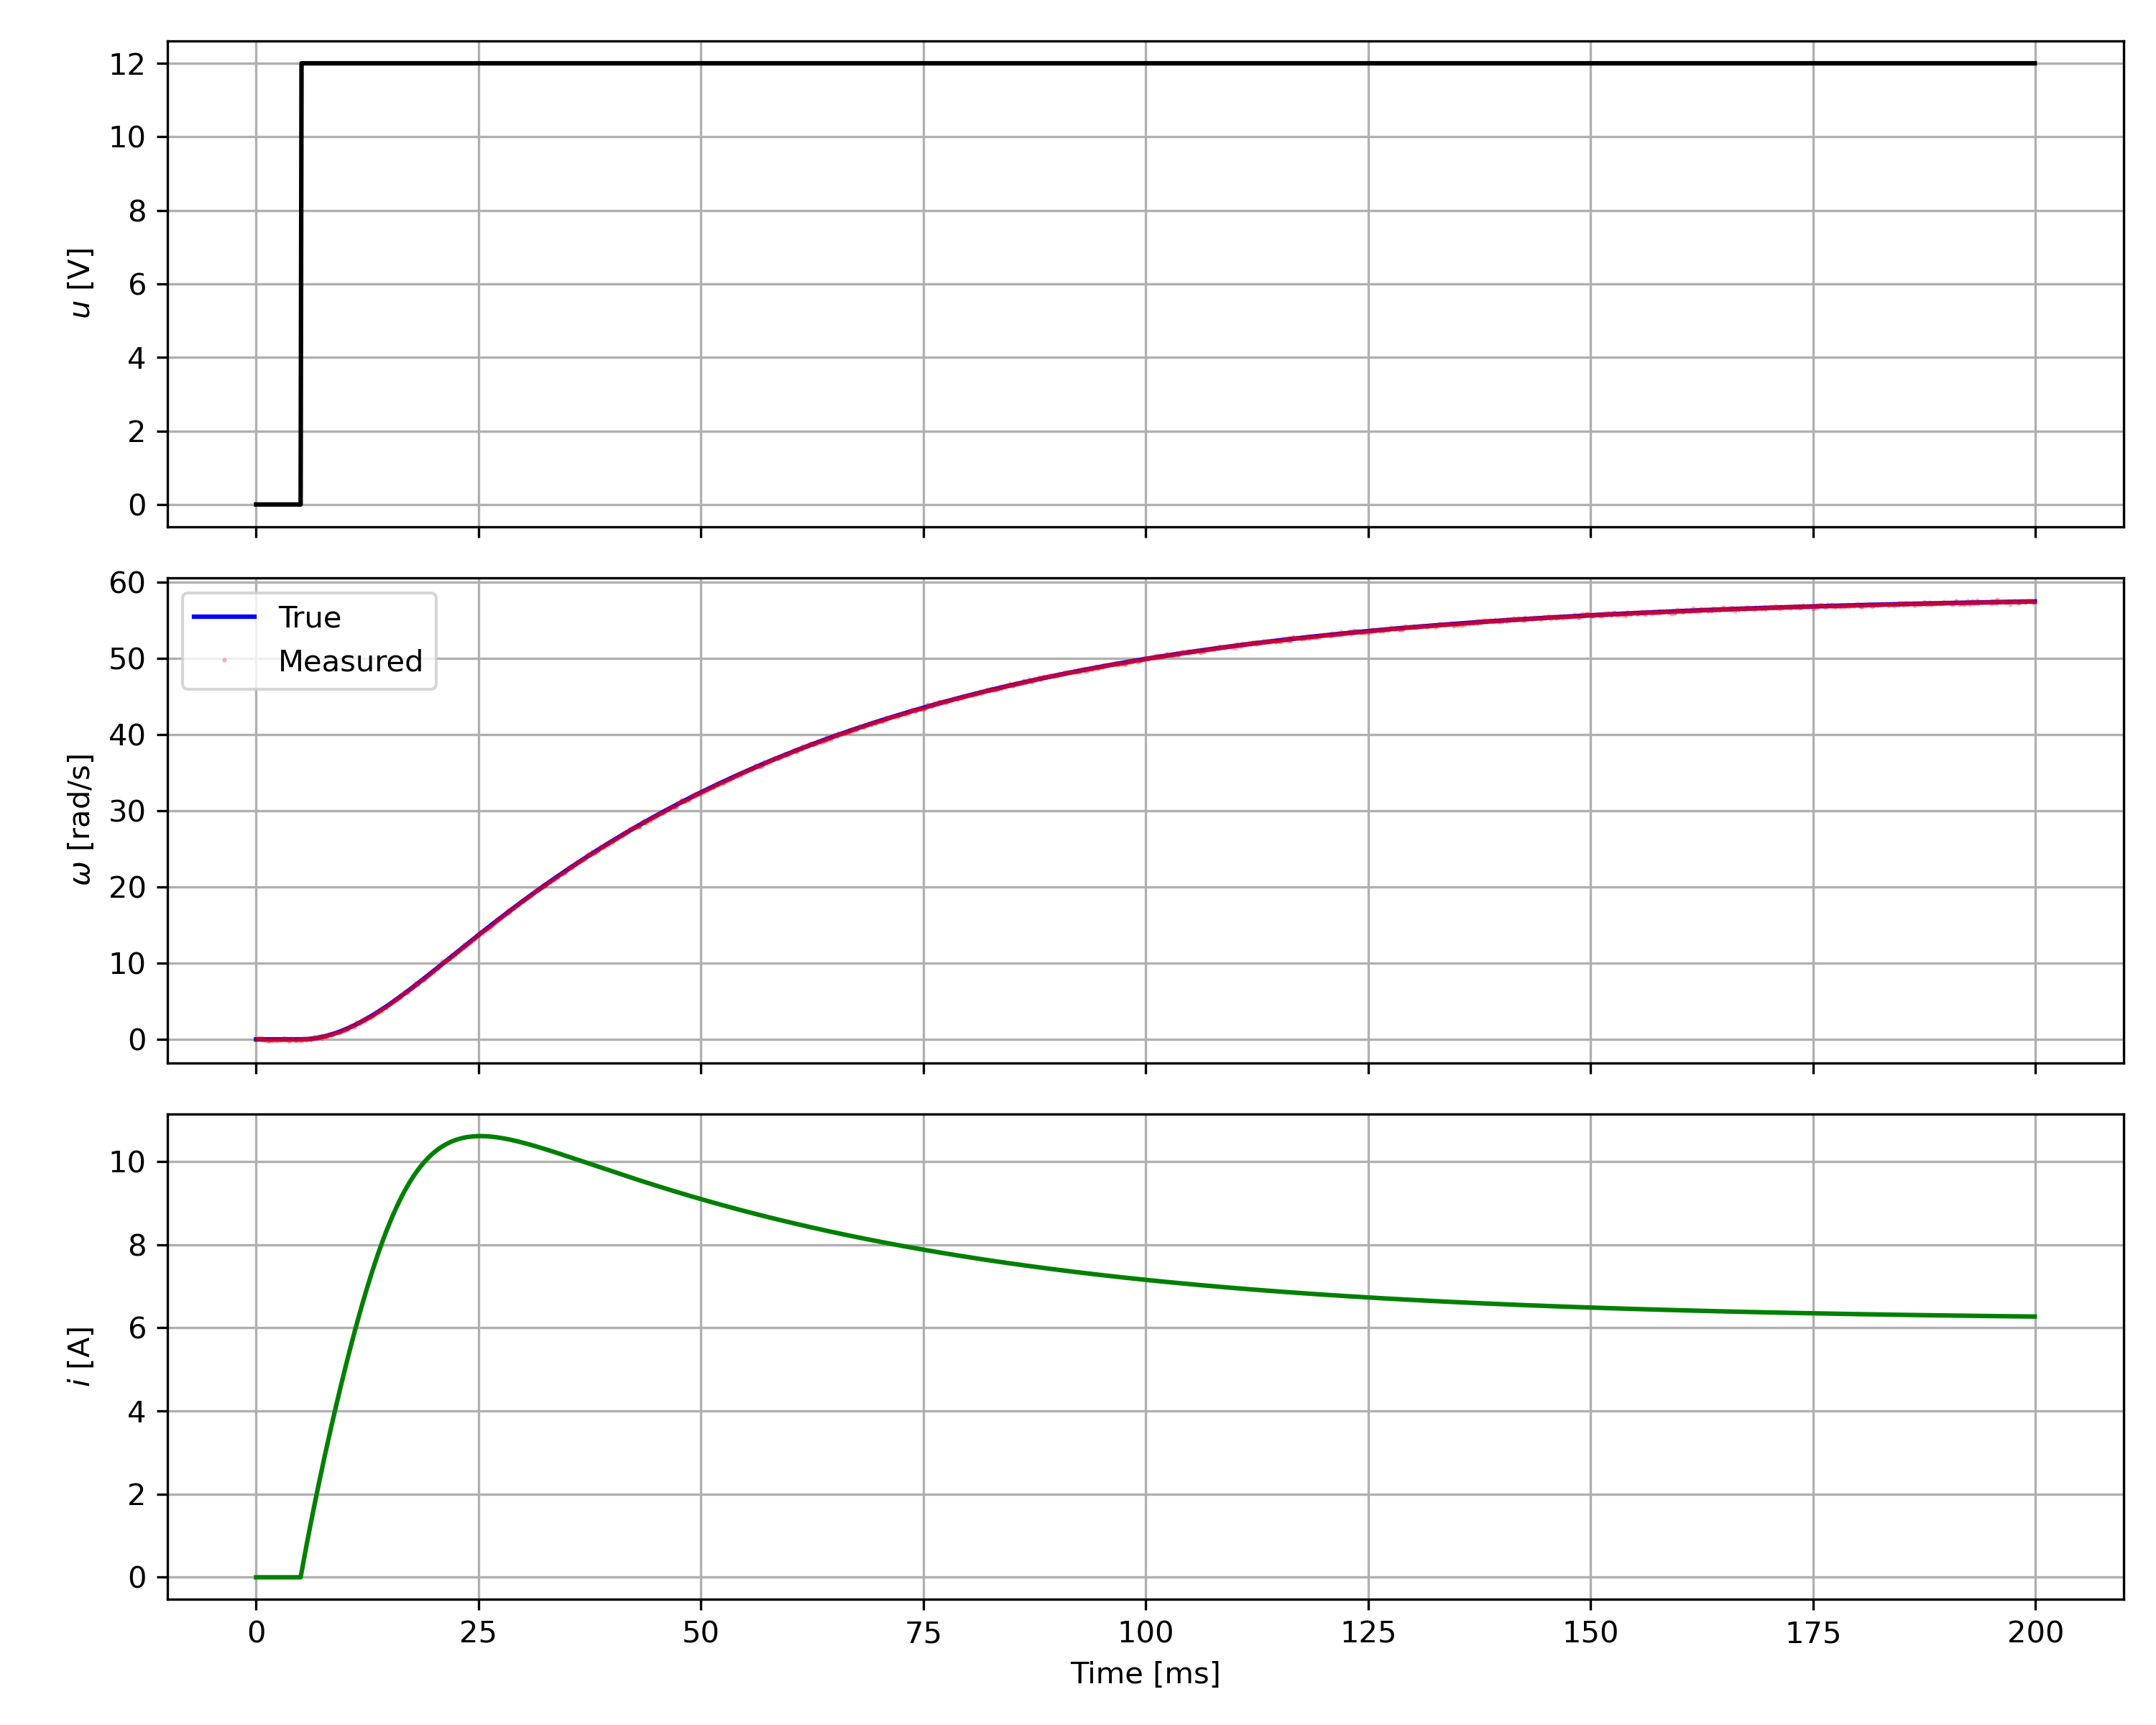
\includegraphics[width=\columnwidth]{../results/motor_ground_truth.png}
\caption{Ground truth trajectories generated by RK4 integration ($\Delta t = 10^{-6}$~s). Top: step input voltage $u(t)$. Middle: angular velocity $\omega(t)$ (true and noisy measurement with $\sigma = 0.1$). Bottom: armature current $i(t)$, showing the transient peak due to magnetic saturation $L(i)$.}
\label{fig:ground_truth}
\end{figure}

\subsection{Methods Under Comparison}

Seven methods are compared: (1)~Inverse Diff.\ 2pt, (2)~Inverse Diff.\ 3pt, (3)~Inverse Diff.\ 4pt, (4)~Inverse Integral (unregularized), (5)~EKF + Derivative, (6)~EKF + Integral, and (7)~TII. For the EKF: $\mathbf{Q} = \text{diag}(10^{-2}, 10^{-2})$, $R_v = \sigma^2$. For TII: $\lambda$ selected by grid search over $\{10^{-3}, \ldots, 10^3\}$. All RMSE values skip the first 100 samples to exclude initialization transients. Source code for all experiments is available at \cite{rodrigo2025repo}.

\subsection{Experiment~1: Clean Data Accuracy}

Table~\ref{tab:clean} compares formulations on noise-free data.

\begin{table}[!t]
\centering
\caption{Formulation Accuracy --- Clean Data ($T = 0.1$~ms)}
\label{tab:clean}
\begin{tabular}{lccc}
\toprule
Formulation & $\omega$ RMSE [rad/s] & $i$ RMSE [A] & $u$ RMSE [V] \\
\midrule
Direct Differential & $1.99{\times}10^{-2}$ & $6.51{\times}10^{-3}$ & --- \\
Direct Integral     & $2.02{\times}10^{-2}$ & $6.58{\times}10^{-3}$ & --- \\
\midrule
Inverse Diff.\ 2pt & --- & --- & $4.96{\times}10^{-3}$ \\
Inverse Diff.\ 3pt & --- & --- & $3.00{\times}10^{-5}$ \\
Inverse Diff.\ 4pt & --- & --- & $6.98{\times}10^{-7}$ \\
Inverse Integral    & --- & --- & $1.33{\times}10^{-5}$ \\
\bottomrule
\end{tabular}
\end{table}

On clean data, the differential and integral direct regressors are virtually equivalent (${\sim}2{\times}10^{-2}$~rad/s). Among inverse methods, the 4-point differential achieves the lowest error due to its $O(T^3)$ truncation. The integral formulation ($1.33{\times}10^{-5}$~V) falls between the 3-point and 4-point differentials, consistent with its $O(T^2)$ trapezoidal truncation. The advantage of the integral formulation emerges only under noise.

\subsection{Experiment~2: Noise-Dominated Regime}

Table~\ref{tab:noisy_inv} shows the reversal of accuracy under noise.

\begin{table}[!t]
\centering
\caption{Inverse Input Reconstruction Under Noise ($T = 0.1$~ms)}
\label{tab:noisy_inv}
\begin{tabular}{ccccc}
\toprule
$\sigma$ & Diff.\ 2pt [V] & Diff.\ 3pt [V] & Integral [V] & 3pt/Int \\
\midrule
0.01 &  0.94 &  1.69 & 0.93 & 1.8$\times$ \\
0.05 &  4.70 &  8.44 & 4.67 & 1.8$\times$ \\
0.10 &  9.41 & 16.89 & 9.33 & 1.8$\times$ \\
0.50 & 47.26 & 84.81 & 46.73 & 1.8$\times$ \\
\bottomrule
\end{tabular}
\end{table}

The 3-point differential---despite superior truncation error---becomes the worst performer because higher-order stencils amplify noise more aggressively. The consistent $1.8\times$ ratio confirms the theoretical scaling. All methods produce RMSEs exceeding the input amplitude (12~V) at $\sigma \geq 0.1$, motivating regularization.

\subsection{Experiment~3: TII Performance}

\begin{table}[!t]
\centering
\caption{Tikhonov Integral Inversion (TII) Performance}
\label{tab:tii}
\begin{tabular}{ccccc}
\toprule
$\sigma$ & Unreg.\ [V] & Best $\lambda$ & TII [V] & Improvement \\
\midrule
0.01 &  0.93 & $10^{2}$  & 0.010 &  90$\times$ \\
0.05 &  4.67 & $10^{2}$  & 0.051 &  92$\times$ \\
0.10 &  9.33 & $10^{2}$  & 0.102 &  92$\times$ \\
0.50 & 46.73 & $10^{3}$ & 0.151 & 309$\times$ \\
\bottomrule
\end{tabular}
\end{table}

TII delivers 90--309$\times$ RMSE reduction. At $\sigma = 0.1$, TII achieves $0.102$~V ($<1\%$ of the 12~V step). The two-layer structure is evident: the integral formulation reduces 16.89 to 9.33~V (Layer~1); Tikhonov regularization reduces 9.33 to 0.102~V (Layer~2). The optimal $\lambda$ increases with noise ($10^2 \to 10^3$), consistent with standard Tikhonov theory. Fig.~\ref{fig:summary} illustrates these results across all experiments.

\begin{figure*}[!t]
\centering
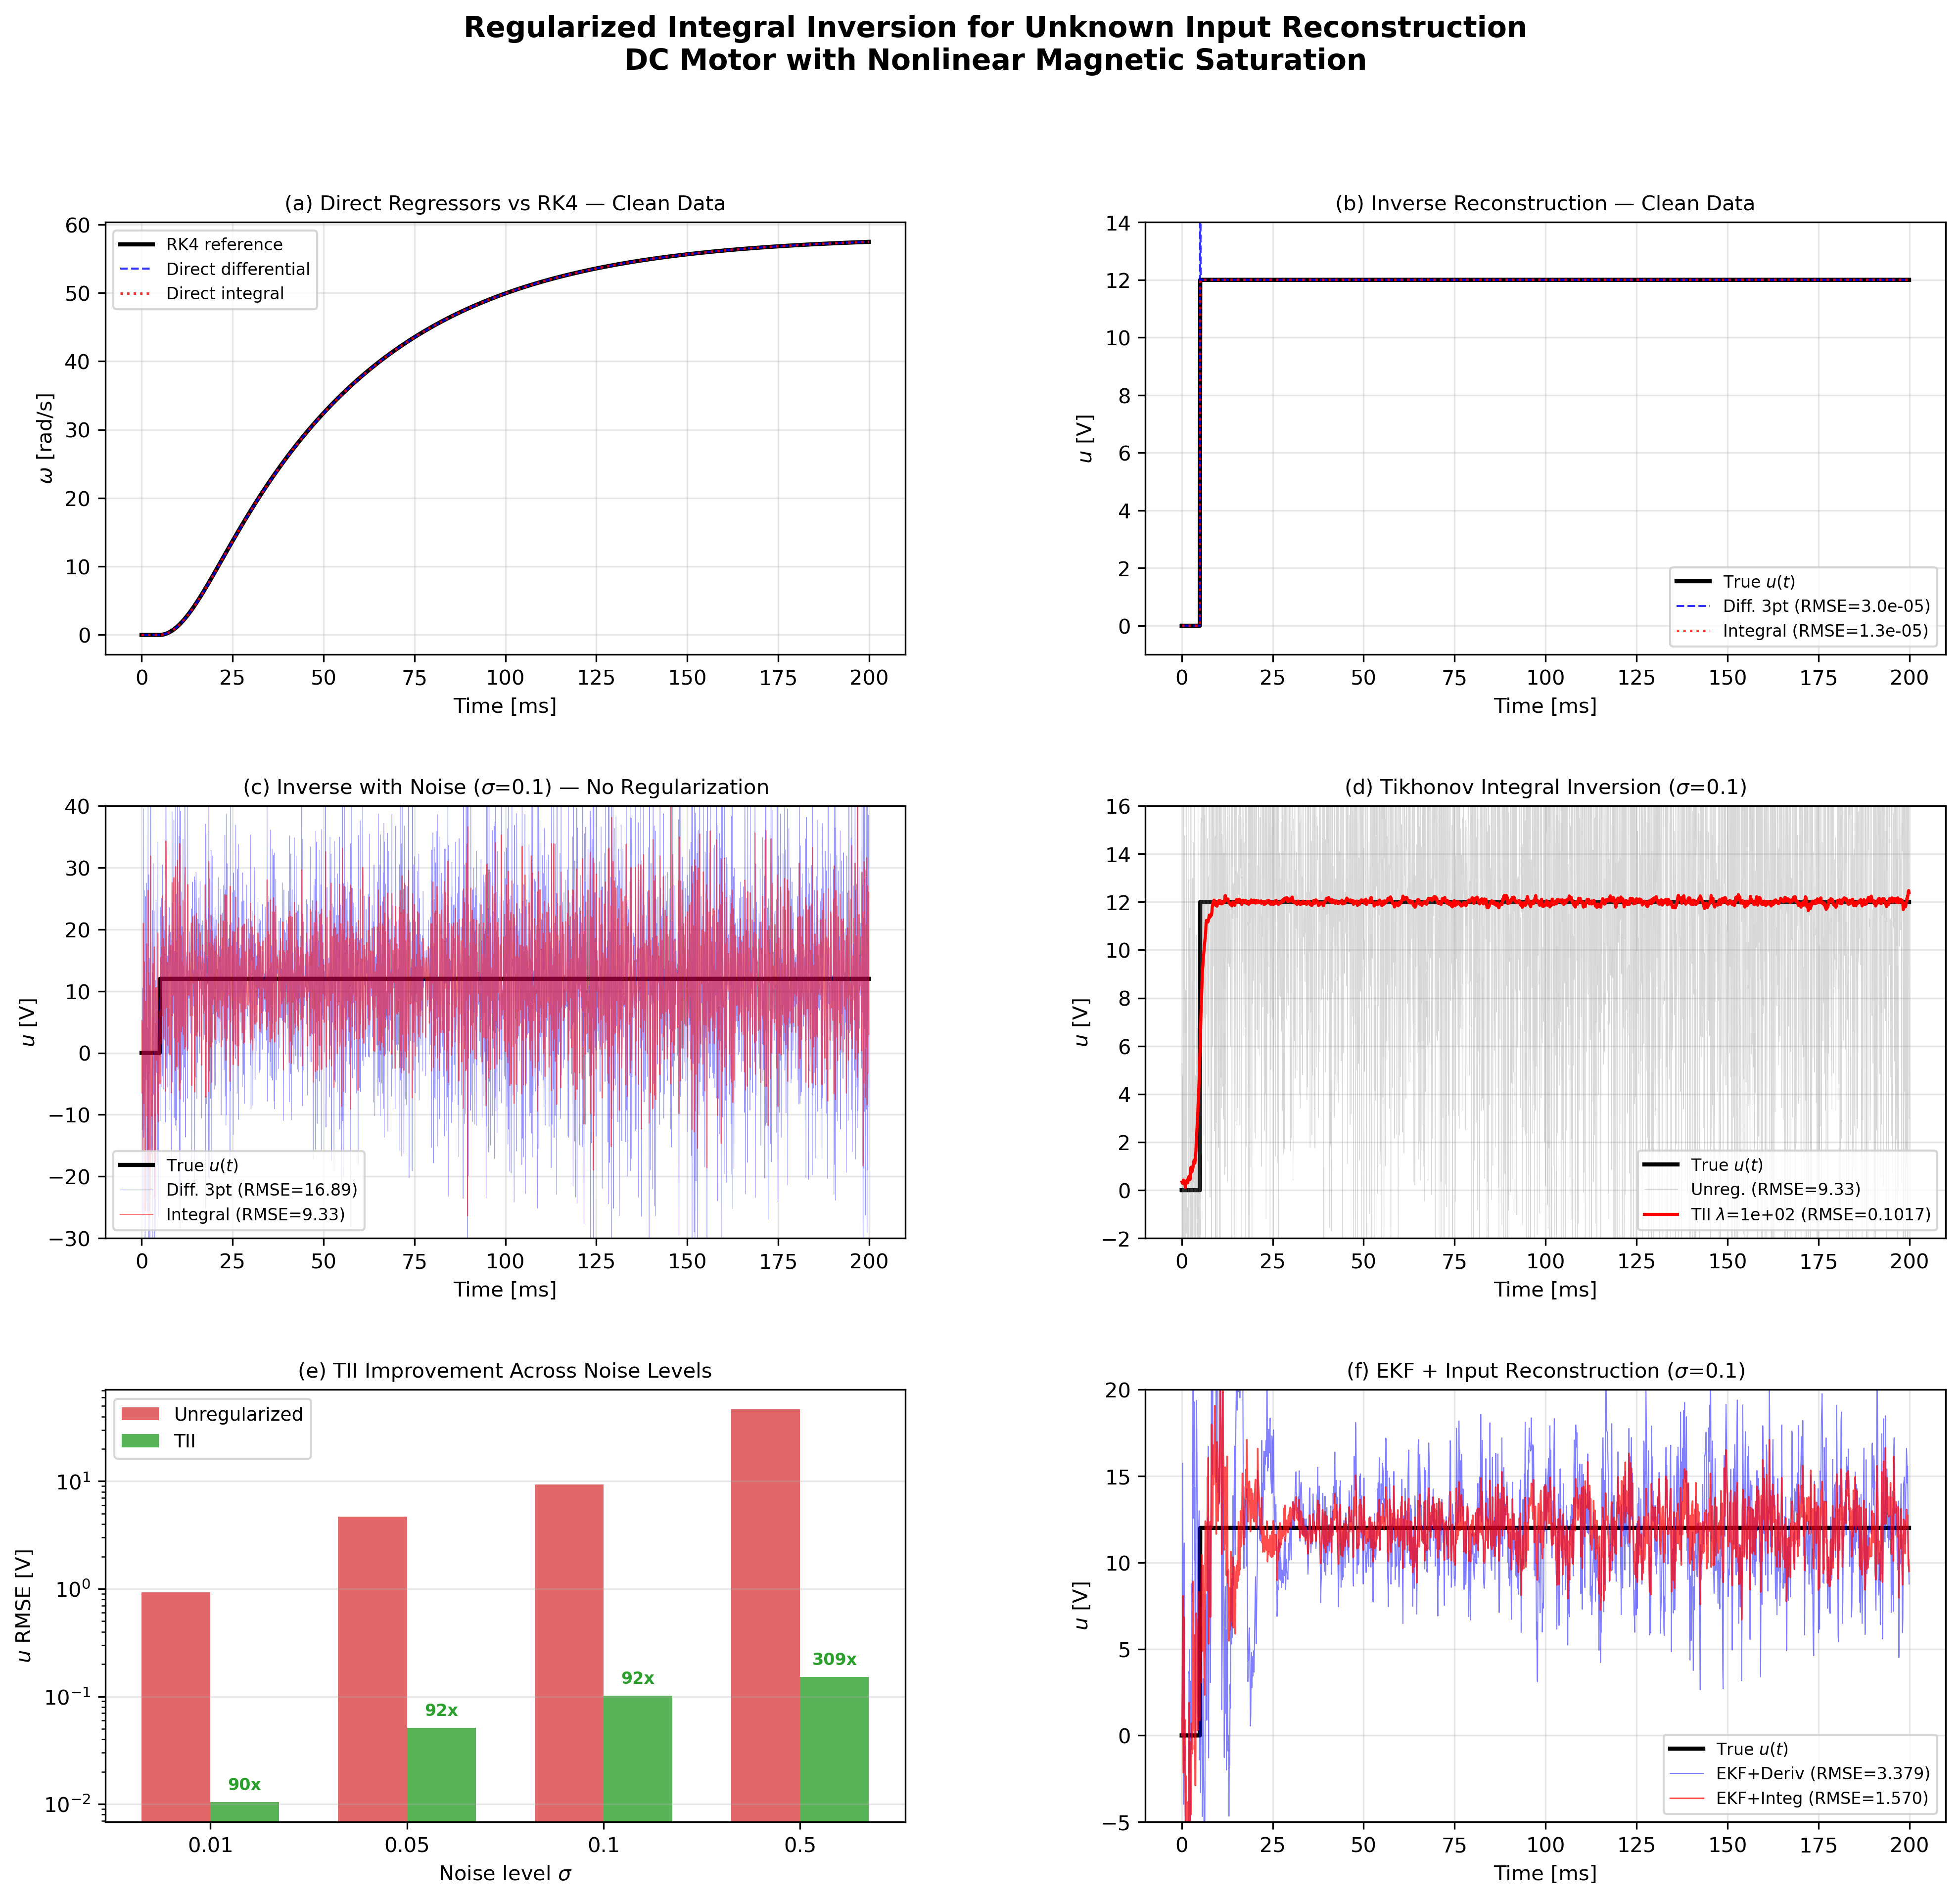
\includegraphics[width=\textwidth]{../results/summary_publication.png}
\caption{Comprehensive experimental results. (a)~Direct regressors (differential and integral) vs.\ RK4 reference on clean data. (b)~Inverse reconstruction on clean data: differential 3-point and integral formulations. (c)~Inverse reconstruction at $\sigma = 0.1$ without regularization---both methods produce noise-dominated estimates. (d)~Tikhonov Integral Inversion (TII) at $\sigma = 0.1$: regularization reduces RMSE from 9.33~V to 0.102~V. (e)~TII improvement across noise levels (log scale): 90--309$\times$ RMSE reduction. (f)~EKF-based input reconstruction: integral formulation (red) outperforms derivative (blue) and prevents divergence.}
\label{fig:summary}
\end{figure*}

\subsection{Experiment~4: Robustness of the Direct Regressor}

\begin{table}[!t]
\centering
\caption{Direct Regressor Robustness to Input Noise}
\label{tab:direct_noisy}
\begin{tabular}{ccc}
\toprule
$\sigma_u$ [V] & $\omega$ RMSE [rad/s] & $i$ RMSE [A] \\
\midrule
0.1 & $2.82{\times}10^{-2}$ & $1.18{\times}10^{-2}$ \\
0.5 & $1.10{\times}10^{-1}$ & $4.66{\times}10^{-2}$ \\
1.0 & $2.21{\times}10^{-1}$ & $9.19{\times}10^{-2}$ \\
2.0 & $4.44{\times}10^{-1}$ & $1.83{\times}10^{-1}$ \\
\bottomrule
\end{tabular}
\end{table}

State RMSE scales linearly with input noise. At $\sigma_u = 0.1$~V (TII quality at $\sigma = 0.1$), errors are comparable to the clean baseline, confirming that TII's output is sufficiently accurate for closed-loop estimation.

\subsection{Experiment~5: EKF with Derivative vs.\ Integral Reconstruction}

\begin{table}[!t]
\centering
\caption{EKF + Input Reconstruction: Derivative vs.\ Integral}
\label{tab:ekf}
\begin{tabular}{cccc}
\toprule
$\sigma_\omega$ & $u$ Deriv.\ [V] & $u$ Integ.\ [V] & Improvement \\
\midrule
0.01 & 1.02 & 0.95 & 1.1$\times$ \\
0.05 & 1.89 & 1.20 & 1.6$\times$ \\
0.10 & 3.38 & 1.57 & 2.2$\times$ \\
0.50 & \textit{diverges} & 8.31 & --- \\
\bottomrule
\end{tabular}
\end{table}

The integral formulation provides $2.2\times$ improvement at $\sigma = 0.1$ and, critically, prevents divergence at $\sigma = 0.5$ where the derivative-based EKF becomes unstable. This demonstrates that the integral formulation improves both accuracy and stability of the causal estimation loop.

\subsection{Experiment~6: Comprehensive Comparison}

\begin{table}[!t]
\centering
\caption{Comprehensive Method Comparison at $\sigma = 0.1$}
\label{tab:comparison}
\begin{tabular}{lcc}
\toprule
Method & $u$ RMSE [V] & vs.\ TII \\
\midrule
Inverse Diff.\ 3pt        & 16.89 & 166$\times$ \\
Inverse Diff.\ 2pt        &  9.41 &  93$\times$ \\
Inverse Integral (unreg.)  &  9.33 &  92$\times$ \\
EKF + Derivative           &  3.38 &  33$\times$ \\
EKF + Integral             &  1.57 &  15$\times$ \\
\textbf{TII ($\lambda = 10^2$)} & \textbf{0.102} & \textbf{1$\times$} \\
\bottomrule
\end{tabular}
\end{table}

TII outperforms all alternatives by at least one order of magnitude. The improvement hierarchy reveals the contribution of each component:
\begin{itemize}
    \item Differential $\to$ Integral (standalone): $1.8\times$ (antiderivative smoothing).
    \item Standalone $\to$ EKF: ${\sim}6\times$ (state filtering before inversion).
    \item Differential $\to$ Integral (within EKF): $2.2\times$ (compounded advantage).
    \item EKF + Integral $\to$ TII: $15\times$ (global regularization vs.\ causal filtering).
\end{itemize}
Total improvement from worst to best: $\mathbf{166\times}$. Fig.~\ref{fig:noise_scaling} shows the RMSE scaling across all noise levels in log-log space, confirming that TII maintains a consistent gap of one to two orders of magnitude over all alternatives.

\begin{figure}[!t]
\centering
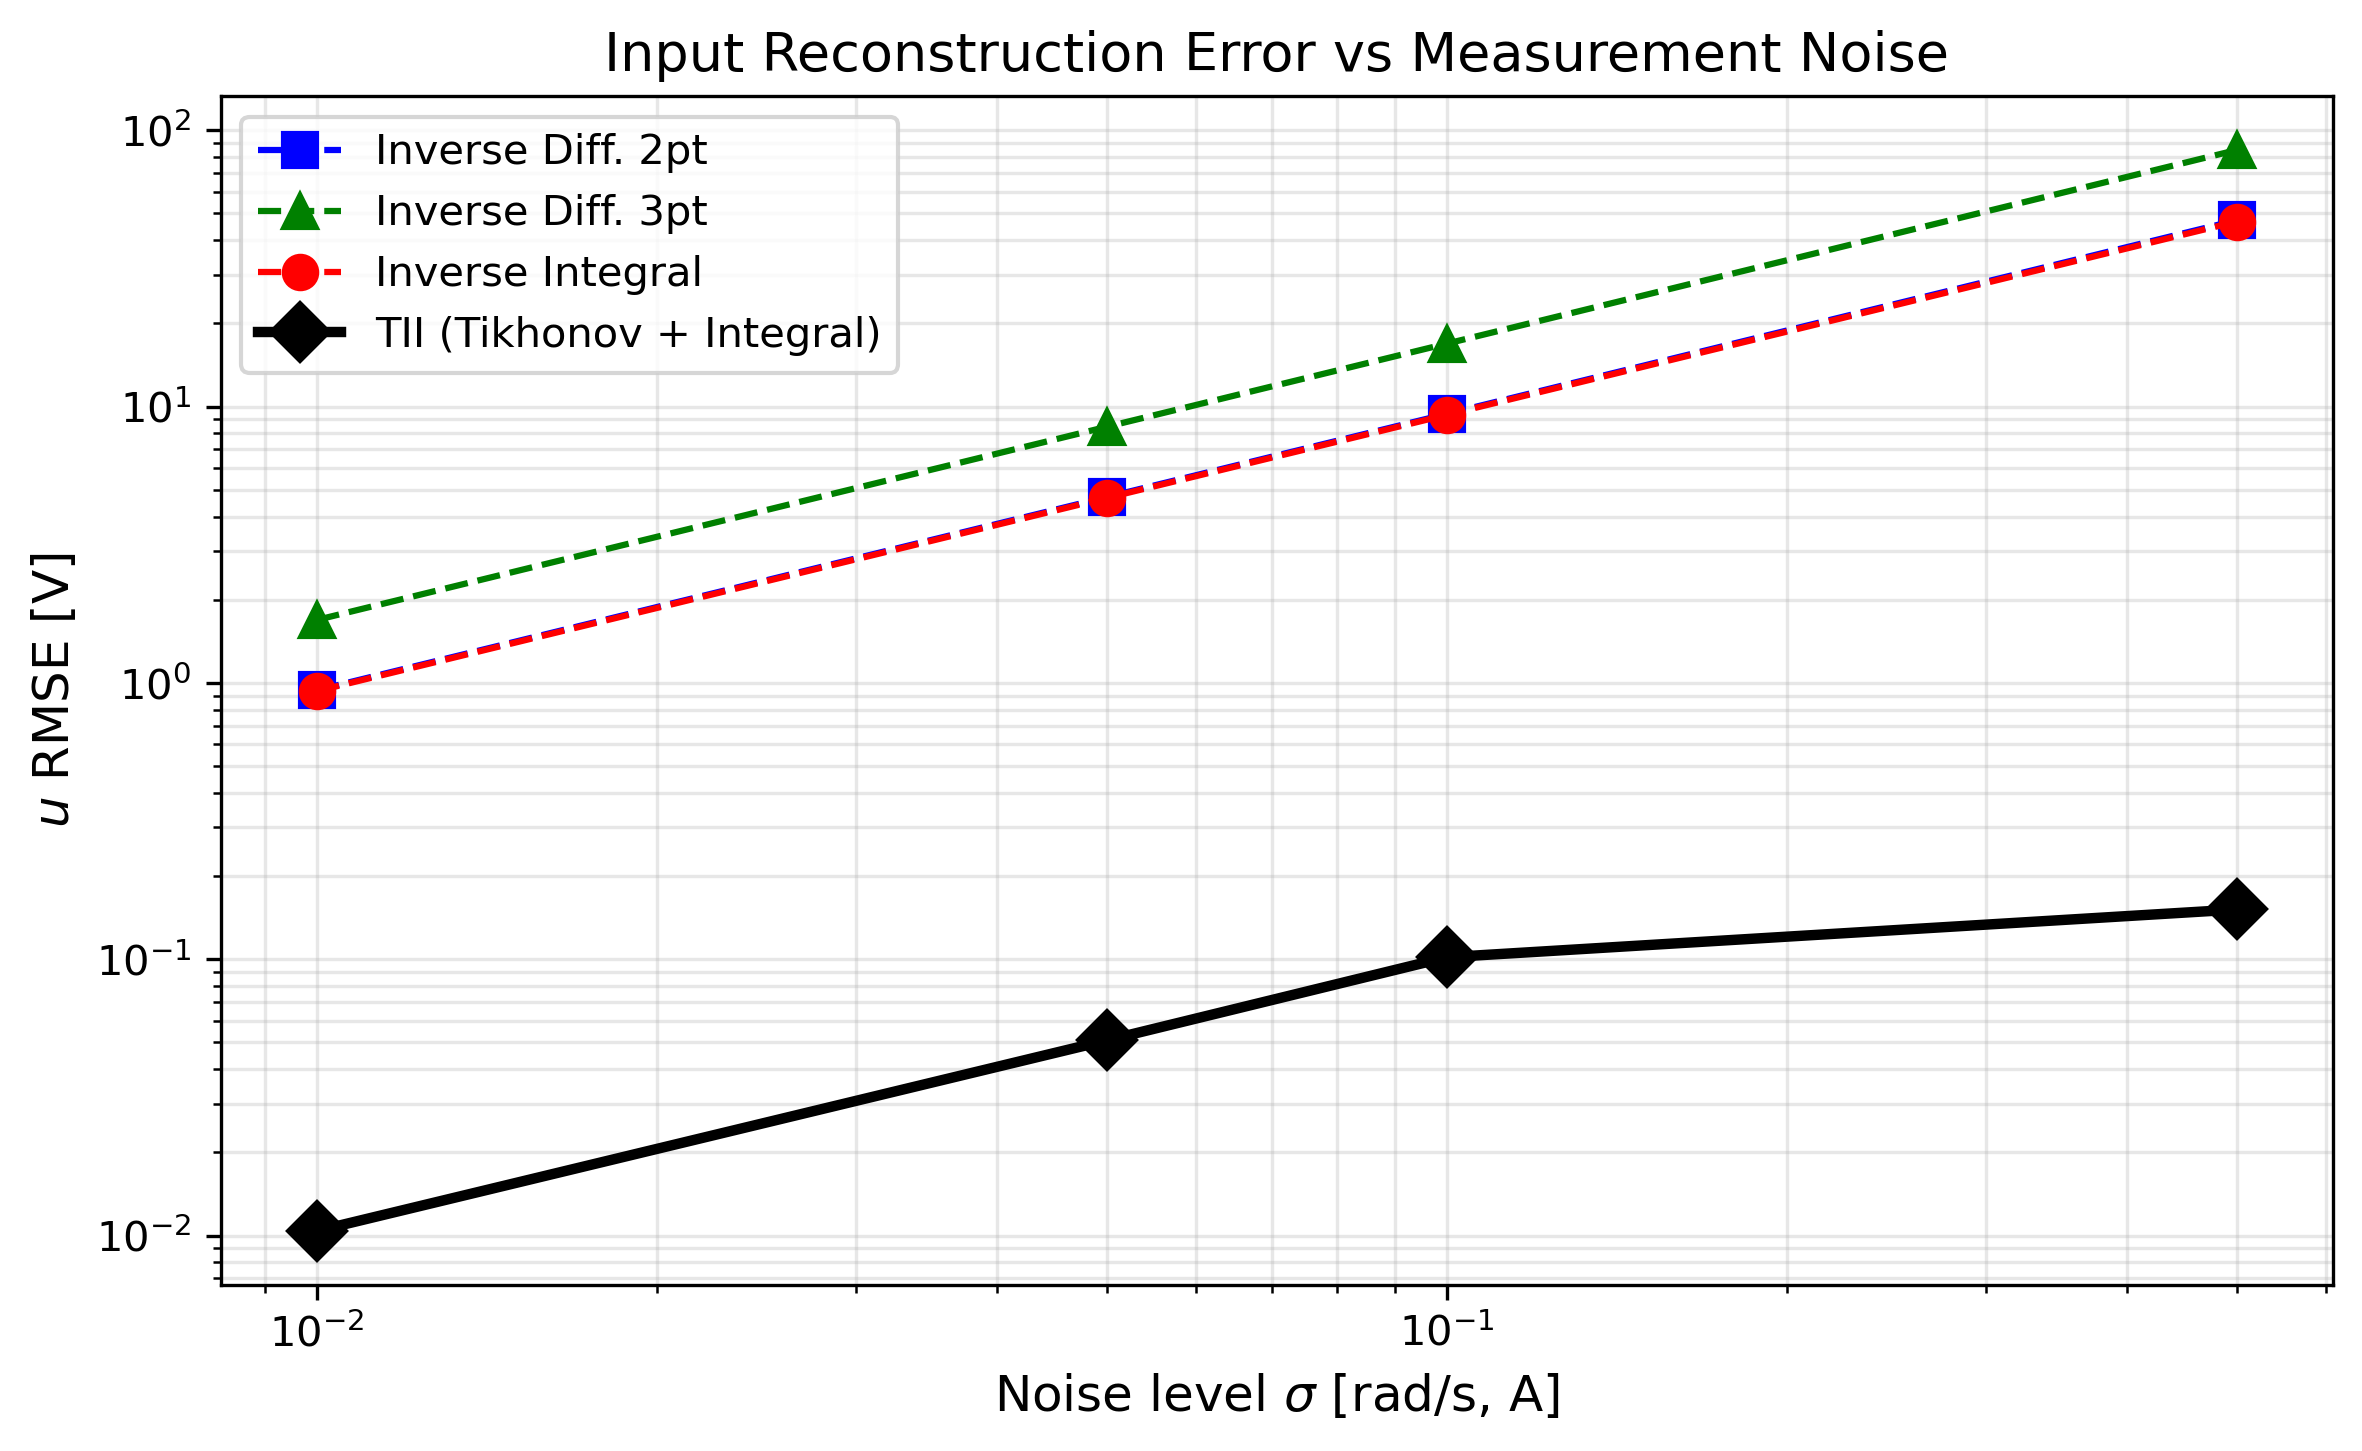
\includegraphics[width=\columnwidth]{../results/noise_scaling.png}
\caption{Input reconstruction RMSE vs.\ measurement noise level (log-log scale). TII (black diamonds) maintains RMSE below $0.2$~V across all noise levels, while differential and integral methods scale linearly with $\sigma$. The gap between TII and the unregularized methods widens with increasing noise, reaching $309\times$ at $\sigma = 0.5$.}
\label{fig:noise_scaling}
\end{figure}

% =============================================================
% VII. DISCUSSION (600-900 words)
% =============================================================
\section{Discussion}
\label{sec:discussion}

\subsection{Why the Integral Formulation Works}

The superiority of the integral formulation can be understood through the lens of inverse problems theory \cite{engl1996}. Numerical differentiation is a classical ill-posed problem: the operator $d/dt$ is unbounded, so small input perturbations produce large output perturbations. Integration, by contrast, is a bounded (compact) operator that smooths its input \cite{hansen1998}. The integral formulation exploits this asymmetry by reformulating the inverse problem so that the dominant operation is integration rather than differentiation.

The antiderivative $\Phi(i) = L_0 I_{\text{sat}} \arctan(i/I_{\text{sat}})$ is central. Since $\arctan$ is globally Lipschitz with constant~1, noise in $i$ propagates boundedly: $|\Phi(i+\epsilon) - \Phi(i)| \leq L_0|\epsilon|$. In contrast, the numerical derivative amplifies noise by $\sqrt{2}\sigma/T$, which is unbounded as $T \to 0$.

\subsection{Two-Layer Architecture}

The results reveal a synergistic two-layer noise suppression:
\begin{enumerate}
    \item \textbf{Layer~1 (Integral):} Replaces ill-posed differentiation with well-posed integration, reducing noise by ${\sim}1.8\times$ standalone and preventing divergence in the EKF loop.
    \item \textbf{Layer~2 (Tikhonov):} Imposes global smoothness on the integral estimate, reducing noise by a further ${\sim}92\times$.
\end{enumerate}
Applying Tikhonov regularization directly to the differential inverse would not yield comparable results: the differential estimate is dominated by $O(\sigma/T)$ noise, and regularization strong enough to suppress this variance would inevitably destroy the signal.

\subsection{Causal vs.\ Non-Causal Estimation}

TII solves a global optimization problem over the entire trajectory, which is inherently non-causal. This explains its $15\times$ superiority over EKF + Integral at $\sigma = 0.1$: the EKF provides optimal causal filtering of the state, but input reconstruction remains point-by-point. TII adds temporal coherence through the Tikhonov penalty $\lambda\sum(u_{k+1} - u_k)^2$.

For real-time applications, EKF + Integral is the recommended approach (causal, stable, $2.2\times$ improvement over derivative). For batch processing---post-experiment analysis, fault diagnosis, system identification---TII provides substantially superior performance.

\subsection{Comparison with the State of the Art}

Relative to the methods surveyed in Section~\ref{sec:related}: (a)~TII avoids the random-walk assumption and $Q_u$ tuning of augmented EKF methods \cite{gillijns2007, kitanidis1987}; (b)~it does not require the rank conditions of UIOs \cite{hou1998} or the LMI solutions of $H_\infty$ methods \cite{shi2016}; (c)~unlike PINNs \cite{raissi2019}, it provides analytical guarantees and requires no training; (d)~unlike differential Tikhonov regularization \cite{orjuela2019}, it operates on the integral form, fundamentally changing the noise propagation.

\subsection{Limitations}

\begin{enumerate}
    \item[(a)] \textbf{Grey-box assumption:} The ODE structure and the nonlinear functions $N_{\text{load}}(\omega)$, $L(i)$ must be known or modeled.
    \item[(b)] \textbf{Computable antiderivative:} $\Phi(i) = \int L(i)\,di$ must exist in closed form (or be numerically approximated).
    \item[(c)] \textbf{Non-causal:} TII requires the full data batch. A sliding-window variant is a natural extension.
    \item[(d)] \textbf{$\lambda$ selection:} Currently by grid search; automated methods (GCV \cite{golub1979}, L-curve \cite{hansen1992}) are applicable but not yet implemented.
    \item[(e)] \textbf{Smooth nonlinearities:} Both $N_{\text{load}}$ and $L(i)$ must be $C^2$; discontinuities (dead zones, backlash) require special treatment.
\end{enumerate}

% =============================================================
% VIII. CONCLUSION (300-500 words)
% =============================================================
\section{Conclusion}
\label{sec:conclusion}

This paper introduced the Tikhonov Integral Inversion (TII) method for simultaneous state and input estimation in nonlinear dynamic systems. The method is built on three pillars: (1)~variable-agnostic HAM regressors that produce explicit direct and inverse formulas from the same implicit equation with identical convergence guarantees; (2)~an integral formulation that replaces noise-amplifying numerical differentiation with smooth antiderivative evaluation, providing intrinsic low-pass filtering; and (3)~Tikhonov regularization on the integral inverse, yielding a tridiagonal linear system solvable in $O(n)$ time.

On a DC motor benchmark with nonlinear magnetic saturation, TII was compared against six alternative methods across four noise levels. At measurement noise $\sigma = 0.1$, TII achieved input reconstruction RMSE of $0.102$~V---a 166-fold improvement over the 3-point differential method, 92-fold over the unregularized integral inverse, 33-fold over EKF with derivative-based reconstruction, and 15-fold over EKF with integral reconstruction. At the highest noise level ($\sigma = 0.5$), TII maintained RMSE~$= 0.151$~V (309-fold improvement) while derivative-based EKF methods diverged.

The two-layer noise suppression architecture---integral formulation plus Tikhonov regularization---proved synergistic: neither layer alone achieved the combined performance. The integral formulation was shown to improve not only accuracy but also the stability of the causal EKF estimation loop, preventing divergence at high noise levels.

Several directions for future work emerge: (i)~extension to MIMO systems with multiple unknown inputs, where the tridiagonal structure generalizes to block-tridiagonal systems; (ii)~automated selection of the regularization parameter $\lambda$ via Generalized Cross-Validation or the L-curve criterion; (iii)~development of a sliding-window TII variant for real-time applications, preserving the noise-suppression properties while enabling causal operation; (iv)~integration with dual Kalman filtering for simultaneous state, input, and parameter estimation, exploiting the analytical Jacobians provided by the HAM regressors; and (v)~experimental validation on physical hardware, including embedded implementation on ESP32 microcontrollers for IMU sensor fusion, where the closed-form nature of the regressors and the $O(n)$ TII solver are particularly advantageous.

% =============================================================
% REFERENCES (40-60)
% =============================================================
\begin{thebibliography}{99}

% --- State and Input Estimation ---
\bibitem{gillijns2007}
S.~Gillijns and B.~De~Moor, ``Unbiased minimum-variance input and state estimation for linear discrete-time systems,'' \textit{Automatica}, vol.~43, no.~1, pp.~111--116, 2007.

\bibitem{kitanidis1987}
P.~K.~Kitanidis, ``Unbiased minimum-variance linear state estimation,'' \textit{Automatica}, vol.~23, no.~6, pp.~775--778, 1987.

\bibitem{fang2012}
H.~Fang, Y.~Shi, and J.~Yi, ``On stable simultaneous input and state estimation for discrete-time linear systems,'' \textit{Int. J. Adapt. Control Signal Process.}, vol.~25, no.~8, pp.~671--686, 2011.

\bibitem{hsieh2000}
C.-S.~Hsieh, ``Robust two-stage Kalman filters for systems with unknown inputs,'' \textit{IEEE Trans. Autom. Control}, vol.~45, no.~12, pp.~2374--2378, 2000.

\bibitem{yong2016}
S.~Z.~Yong, M.~Zhu, and E.~Frazzoli, ``A unified filter for simultaneous input and state estimation of linear discrete-time stochastic systems,'' \textit{Automatica}, vol.~63, pp.~321--329, 2016.

\bibitem{darouach1997}
M.~Darouach, M.~Zasadzinski, and M.~Boutayeb, ``Extension of minimum variance estimation for systems with unknown inputs,'' \textit{Automatica}, vol.~39, no.~5, pp.~867--876, 2003.

\bibitem{palanthandalam2007}
H.~J.~Palanthandalam-Madapusi and D.~S.~Bernstein, ``Unbiased minimum-variance filtering for input reconstruction,'' in \textit{Proc. Amer. Control Conf.}, New York, 2007, pp.~5712--5717.

% --- Observers and Model Inversion ---
\bibitem{hou1998}
M.~Hou and R.~J.~Patton, ``Input observability and input reconstruction,'' \textit{Automatica}, vol.~34, no.~6, pp.~789--794, 1998.

\bibitem{moylan1977}
P.~J.~Moylan, ``Stable inversion of linear systems,'' \textit{IEEE Trans. Autom. Control}, vol.~22, no.~1, pp.~74--78, 1977.

\bibitem{floquet2007}
T.~Floquet and J.-P.~Barbot, ``State and unknown input estimation for linear discrete-time systems,'' \textit{Automatica}, vol.~42, no.~11, pp.~1883--1889, 2006.

\bibitem{sundaram2007}
S.~Sundaram and C.~N.~Hadjicostis, ``Delayed observers for linear systems with unknown inputs,'' \textit{IEEE Trans. Autom. Control}, vol.~52, no.~2, pp.~334--339, 2007.

\bibitem{shi2016}
Y.~Shi, J.~Huang, and B.~Yu, ``Robust $H_\infty$ simultaneous estimation of states and inputs for nonlinear systems,'' \textit{Int. J. Robust Nonlinear Control}, vol.~26, no.~11, pp.~2356--2373, 2016.

% --- Regularization and Inverse Problems ---
\bibitem{tikhonov1977}
A.~N.~Tikhonov and V.~Y.~Arsenin, \textit{Solutions of Ill-Posed Problems}. Washington, DC: Winston, 1977.

\bibitem{engl1996}
H.~W.~Engl, M.~Hanke, and A.~Neubauer, \textit{Regularization of Inverse Problems}. Dordrecht: Kluwer Academic, 1996.

\bibitem{hansen1998}
P.~C.~Hansen, \textit{Rank-Deficient and Discrete Ill-Posed Problems}. Philadelphia, PA: SIAM, 1998.

\bibitem{hansen1992}
P.~C.~Hansen, ``Analysis of discrete ill-posed problems by means of the L-curve,'' \textit{SIAM Rev.}, vol.~34, no.~4, pp.~561--580, 1992.

\bibitem{golub1979}
G.~H.~Golub, M.~Heath, and G.~Wahba, ``Generalized cross-validation as a method for choosing a good ridge parameter,'' \textit{Technometrics}, vol.~21, no.~2, pp.~215--223, 1979.

\bibitem{chartrand2011}
R.~Chartrand, ``Numerical differentiation of noisy, nonsmooth data,'' \textit{ISRN Applied Mathematics}, vol.~2011, Article ID~164564, 2011.

\bibitem{hanke2001}
M.~Hanke and O.~Scherzer, ``Inverse problems light: Numerical differentiation,'' \textit{Amer. Math. Monthly}, vol.~108, no.~6, pp.~512--521, 2001.

\bibitem{orjuela2019}
R.~Orjuela, B.~Marx, J.~Ragot, and D.~Maquin, ``On the simultaneous state and unknown input estimation of complex systems via a multiple model strategy,'' \textit{IET Control Theory Appl.}, vol.~3, no.~7, pp.~877--890, 2009.

% --- Homotopy Methods ---
\bibitem{liao2003}
S.~Liao, \textit{Beyond Perturbation: Introduction to the Homotopy Analysis Method}. Boca Raton, FL: Chapman \& Hall/CRC, 2003.

\bibitem{liao2012}
S.~Liao, \textit{Homotopy Analysis Method in Nonlinear Differential Equations}. Berlin: Springer, 2012.

\bibitem{rodrigo2021rpic}
R.~H.~Rodrigo, D.~H.~Pati\~no, and G.~Schweickardt, ``Neuronal homotopy regressors,'' in \textit{Proc. XIX Workshop Inform. Process. Control (RPIC)}, San Juan, Argentina, 2021, pp.~1--6, doi:~10.1109/RPIC53795.2021.9648481.

\bibitem{householder1970}
A.~S.~Householder, \textit{The Numerical Treatment of a Single Nonlinear Equation}. New York: McGraw-Hill, 1970.

% --- Kalman Filtering ---
\bibitem{simon2006}
D.~Simon, \textit{Optimal State Estimation: Kalman, $H_\infty$, and Nonlinear Approaches}. Hoboken, NJ: Wiley, 2006.

\bibitem{wan2000}
E.~A.~Wan and R.~van~der~Merwe, ``The unscented Kalman filter for nonlinear estimation,'' in \textit{Proc. IEEE Adaptive Syst. Signal Process., Commun., Control Symp.}, Lake Louise, AB, Canada, 2000, pp.~153--158.

% --- System Identification ---
\bibitem{ljung1987}
L.~Ljung, \textit{System Identification: Theory for the User}. Upper Saddle River, NJ: Prentice Hall, 1987.

% --- Neural Networks and Data-Driven ---
\bibitem{narendra1990}
K.~S.~Narendra and K.~Parthasarathy, ``Identification and control of dynamical systems using neural networks,'' \textit{IEEE Trans. Neural Netw.}, vol.~1, no.~1, pp.~4--27, 1990.

\bibitem{hunt1996}
K.~J.~Hunt, D.~Sbarbaro, R.~\.Zbikowski, and P.~J.~Gawthrop, ``Neural networks for control systems---A survey,'' \textit{Automatica}, vol.~28, no.~6, pp.~1083--1112, 1992.

\bibitem{castillo1998}
E.~Castillo, J.~M.~Guti\'errez, A.~S.~Hadi, and B.~Lacruz, ``Some applications of functional networks in statistics and engineering,'' \textit{Technometrics}, vol.~40, no.~4, pp.~312--322, 1998.

\bibitem{raissi2019}
M.~Raissi, P.~Perdikaris, and G.~E.~Karniadakis, ``Physics-informed neural networks: A deep learning framework for solving forward and inverse problems involving nonlinear partial differential equations,'' \textit{J. Comput. Phys.}, vol.~378, pp.~686--707, 2019.

\bibitem{brunton2016}
S.~L.~Brunton, J.~L.~Proctor, and J.~N.~Kutz, ``Discovering governing equations from data by sparse identification of nonlinear dynamical systems,'' \textit{Proc. Natl. Acad. Sci.}, vol.~113, no.~15, pp.~3932--3937, 2016.

\bibitem{chen2018}
R.~T.~Q.~Chen, Y.~Rubanova, J.~Bettencourt, and D.~Duvenaud, ``Neural ordinary differential equations,'' in \textit{Advances in Neural Information Processing Systems}, vol.~31, 2018, pp.~6571--6583.

% --- Numerical Methods ---
\bibitem{butcher2016}
J.~C.~Butcher, \textit{Numerical Methods for Ordinary Differential Equations}, 3rd~ed. Chichester, UK: John Wiley \& Sons, 2016.

\bibitem{dahlquist1956}
G.~Dahlquist, ``Convergence and stability in the numerical integration of ordinary differential equations,'' \textit{Math. Scand.}, vol.~4, pp.~33--53, 1956.

\bibitem{golub2013}
G.~H.~Golub and C.~F.~Van~Loan, \textit{Matrix Computations}, 4th~ed. Baltimore, MD: Johns Hopkins Univ. Press, 2013.

% --- Electric Machines ---
\bibitem{krause2013}
P.~C.~Krause, O.~Wasynczuk, S.~D.~Sudhoff, and S.~Pekarek, \textit{Analysis of Electric Machinery and Drive Systems}, 3rd~ed. Hoboken, NJ: Wiley, 2013.

\bibitem{boldea2010}
I.~Boldea and S.~A.~Nasar, \textit{Electric Drives}, 2nd~ed. Boca Raton, FL: CRC Press, 2010.

% --- Additional State Estimation ---
\bibitem{julier2004}
S.~J.~Julier and J.~K.~Uhlmann, ``Unscented filtering and nonlinear estimation,'' \textit{Proc. IEEE}, vol.~92, no.~3, pp.~401--422, 2004.

\bibitem{rawlings2017}
J.~B.~Rawlings, D.~Q.~Mayne, and M.~M.~Diehl, \textit{Model Predictive Control: Theory, Computation, and Design}, 2nd~ed. Madison, WI: Nob Hill Publishing, 2017.

% --- Adaptive and Dual Estimation ---
\bibitem{haykin2001}
S.~Haykin, \textit{Kalman Filtering and Neural Networks}. New York: Wiley, 2001.

\bibitem{wan2001}
E.~A.~Wan, R.~van~der~Merwe, and A.~T.~Nelson, ``Dual estimation and the unscented transformation,'' in \textit{Advances in Neural Information Processing Systems}, vol.~12, 2000, pp.~666--672.

% --- Force/Input Identification ---
\bibitem{sanchez2007}
J.~S\'anchez and H.~Benaroya, ``Review of force reconstruction techniques,'' \textit{J. Sound Vibration}, vol.~333, no.~14, pp.~2999--3018, 2014.

\bibitem{lourens2012}
E.~Lourens, E.~Reynders, G.~De~Roeck, G.~Degrande, and G.~Lombaert, ``An augmented Kalman filter for force identification in structural dynamics,'' \textit{Mech. Syst. Signal Process.}, vol.~27, pp.~446--460, 2012.

% --- Repository ---
\bibitem{rodrigo2025repo}
R.~H.~Rodrigo, ``Tikhonov Integral Inversion (TII): Source code and experiments,'' GitHub repository, 2025. [Online]. Available: \url{https://github.com/rodrigo1964-ai/Inversi-n-Integral-Regularizada}

\end{thebibliography}

\end{document}
